
\section{Monday for MAT3006}\index{Monday_lecture}


\paragraph{Reviewing}
We define the \emph{outer} measure of a subset $E\subseteq\mathbb{R}$ to be
\[
m^*(E)
=
\inf\left\{
\sum_{n=1}^\infty m(I_n)
\middle|
E\subseteq\bigcup_{n=1}^\infty I_n,\ \text{$I_n$'s are open intervals}
\right\}
\]
One Special Property of Outer Measure:
\[
m^*(\cup_{n=1}^\infty E_n)\le\sum_{n=1}^\infty m^*(E_n)
\]
\subsection{Remarks for Outer Measure}
We want to make a special hyphothesis become true:
If $E_n$'s are disjoint, then
\begin{equation}\label{Eq:8:3}
m^*(\cup_{n=1}^\infty E_n)=\sum_{n=1}^\infty m^*(E_n)
\end{equation}
However, (\ref{Eq:8:3}) does not necessary hold for a sequence of disjoint subsets $\{E_n\}$.
One counter-example is shown in Example~(\ref{exp:8:2}).

\begin{example}[Vitali Set]\label{exp:8:2}
Suppose that $A\subseteq[0,1]$ satisfies the following properties:
\begin{itemize}
\item
For any $x\in\mathbb{R}$,
there exists $q\in\mathbb{Q}$ such that
$x+q\in A$.
\item
If $x,y\in A$ such that $x\ne y$, then $x-y\notin\mathbb{Q}$
\end{itemize}
In other words, 
the group $\mathbb{R}$ is partitioned into the cosets of its additive subgroup $\mathbb{Q}$, and the properties above say that $A$ contains exactly one member of each coset of $\mathbb{Q}$.
The existence of such $A$ relies on the Axiom of Choice.
Moreover, we imply:
\begin{itemize}
\item
$[0,1]\subseteq\bigcup_{q\in[-1,1]\cap\mathbb{Q}}(A-q)$:
since $\forall x\in[0,1]$, there exists $q\in\mathbb{Q}$ s.t. $x+q\in A$, which implies $x\in A-q$.
Moreover, we can bound the possible region of $q$:
\[
0\le x+q\le 1\implies -x\le q\le 1-x\implies -1\le q\le 1
\]
\item
$\bigcup_{q\in[-1,1]\cap\mathbb{Q}}(A-q)\subseteq[-1,2]$:
elements in $A-q$ are of the form $x-q, x\in[0,1],q\in[-1,1]$, and therefore $x-q\in[-1,2]$.
\item
The sets $(A-q)$ are disjoint as $q$ varies, i.e., $(A-q_1)\cap(A-q_2)=\emptyset,\forall q_1\ne q_2\in[-1,1]\cap\mathbb{Q}$:
Suppose on the contrary that there exists $y\in (A-q_1)\cap(A-q_2)$, which follows
\[
y+q_1,y+q_2\in A,
y+q_1\ne y+q_2\implies
(y+q_1)-(y+q_2)=q_1-q_2\notin\mathbb{Q}
\]
\end{itemize}
Suppose on the contrary that (\ref{Eq:8:3}) holds for $\{A-q\mid\forall q\in[-1,1]\cap\mathbb{Q}\}$, then
\begin{equation}\label{Eq:8:4}
m^*\left(\bigcup_{q\in[-1,1]\cap\mathbb{Q}}(A-q)\right)=\sum_{q\in[-1,1]\cap\mathbb{Q}}m^*(A-q)=\sum_{q\in[-1,1]\cap\mathbb{Q}}m^*(A),
\end{equation}
where the second equality is because that $m^*(A-q)=m^*(A),\forall q$.
However,
\begin{equation}\label{Eq:8:5}
1=m^*([0,1])\le m^*\left(\bigcup_{q\in[-1,1]\cap\mathbb{Q}}(A-q)\right)\le m^*([-1,2])=3
\end{equation}
From (\ref{Eq:8:4}) we derive the $m^*\left(\bigcup_{q\in[-1,1]\cap\mathbb{Q}}(A-q)\right)$ can either be $0$ or $\infty$, which is a contradiction.
\end{example}
\subsection{Lebesgue Measurable}
Therefore, (\ref{Eq:8:5}) does not hold for some bad subsets of $\mathbb{R}$, which are sets cannot be explicitly described.
Let's focus on sets with good behaviour only:
\begin{definition}[Carathedory Property]\label{def:8:2}
A subset $E\subseteq\mathbb{R}$ is \emph{measurable} if 
\begin{equation}\label{Eq:8:6}
m^*(A)=m^*(A\cap E)+m^*(A\setminus E)
\end{equation}
for all subsets $A\subseteq\mathbb{R}$, where $E$ is not assumed to be in $A$, i.e., $A\setminus E:=A\cap E^c$.
\end{definition}
\begin{remark}
To argue whether (\ref{Eq:8:6}) holds, we essentially suffice to verify the inequality $m^*(A)\ge m^*(A\cap E)+m^*(A\setminus E)$.
There are many other equivalent definitions for measurable set $E\subseteq\mathbb{R}$:
\begin{enumerate}
\item
For any $\varepsilon>0$, there exists open set $U\supseteq E$ such that 
\[
m^*(U\setminus E)\le\varepsilon
\]
\item
Its outer and inner measures are equal:
\[
m^*(E)=m_*(E):=\sup\left\{\sum_{n=1}^\infty m(I_n)\middle|\bigcup_{n=1}^\infty I_n\subseteq E,\ \text{$I_n$'s are compact, and disjoint subsets}\right\}
\]
Note that the inner measure $m_*$ admits the inequality
\[
m_*(\cup_{n=1}^\infty E_n)\ge\sum_{n=1}^\infty m_*(E_n),\ \text{for disjoint $E_n$}
\]

\end{enumerate}
\end{remark}

\begin{remark}
If $E\subseteq\mathbb{R}$, then for all $B\supseteq E$, we have
\begin{equation}\label{Eq:8:7}
m^*(B) = m^*(B\cap E)+m^*(B\setminus E) = m^*(E) + m^*(B\setminus E):
\end{equation}
\begin{figure}[H]
\centering
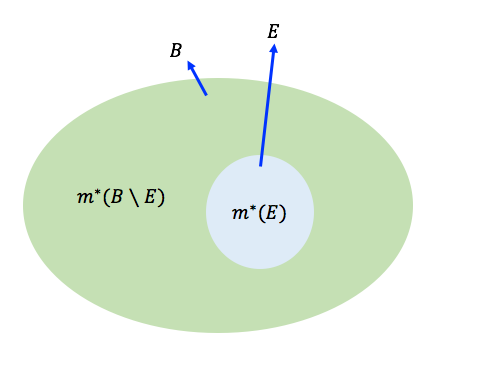
\includegraphics[width=0.5\textwidth]{week7/p_1}
\caption{Illustration for the useful equality (\ref{Eq:8:7})}
\end{figure}
\end{remark}

\begin{proposition}
\begin{enumerate}
\item
If $E\subseteq\mathbb{R}$ is null, then $E$ is measurable
\item
If $I$ is any interval, then $I$ is measurable
\item
If $E$ is measurable, then $E^c:=\mathbb{R}\setminus E$ is measurable
\item
If $E$ is measurable, then both $\cup_{i=1}^nE_i$ and $\cap_{i=1}^nE_i$ are measurable
\end{enumerate}
\end{proposition}

\begin{proof}
\begin{enumerate}
\item
For any subsets $A$,
\[
\left\{
\begin{aligned}
m^*(A\cap E)&=0\\
m^*(A\cap E^c)&\le m^*(A)
\end{aligned}
\right.
\implies m^*(A)\ge m^*(A\cap E)+m^*(A\cap E^c).
\]
\item
Take $I=[a,b]$. For all $A\subseteq\mathbb{R}$,
\begin{itemize}
\item
take $\{I_n\}$ such that $A\subseteq\cup_{n=1}^\infty I_n$ and
\begin{equation}\label{Eq:8:8}
\sum_{n=1}^\infty m^*(I_n)\le m^*(A)+\varepsilon
\end{equation}
\item
Note that the $m^*(A\cap I)$ can be upper bounded:
\[
A\cap I\subseteq \cup_{n=1}^\infty (I_n\cap I)\implies
m^*(A\cap I)\le \sum_{n=1}^\infty m^*(I_n\cap[a,b])
\]
Similarly, $m^*(A\cap I^c)$ can be upper bounded:
\[
A\cap I^c \subseteq\cup_{n=1}^\infty I_n\cap((-\infty ,a)\cup(b,\infty))
=
\left(\bigcup_{n=1}^\infty I_n\cap (-\infty,a)\right)
\cup
\left(\bigcup_{n=1}^\infty I_n\cap (b,\infty)\right),
\]
i.e.,
\[
m^*(A\cap I^c)\le \sum_{n=1}^\infty m^*(I_n\cap(-\infty,a))
+m^*(I_n\cap(b,\infty))
\]
\item
Therefore,
\begin{align*}
m^*(A\cap I)+m^*(A\cap I^c)
&\le
\sum_{n=1}^\infty m^*(I_n\cap(-\infty,a))+m^*(I_n\cap[a,b])
+m^*(I_n\cap(b,\infty))\\&=
\sum_{n=1}^\infty
m^*(I_n\cap(-\infty,\infty))=
\sum_{n=1}^\infty
m^*(I_n)\\
&\le m^*(A)+\varepsilon,
\end{align*}
i.e., $m^*(A\cap I)+m^*(A\cap I^c)\le m^*(A)$.
\end{itemize}

\item
Part~(3) is trivial.
\item
Part~(4) is by induction on $n$:
suppose that
\begin{itemize}
\item
$E_i$ is measurable for $i=1,\dots,k+1$
\item
$E=\cup_{i=1}^kE_i$ is measurable
\end{itemize}
By the measurablitiy of $E_{k+1}$,
\begin{equation}\label{Eq:8:9}
m^*(A\cap E^c) = m^*(A\cap E^c\cap E_{k+1})+m^*(A\cap E^c\cap E_{k+1}^c)
\end{equation}
By the measurablitiy of $E$,
\begin{equation}\label{Eq:8:10}
\begin{aligned}
m^*(A)&\ge m^*(A\cap E)+m^*(A\cap E^c)\\&\ge
 [m^*(A\cap E)+m^*(A\cap E^c\cap E_{k+1})]+m^*(A\cap E^c\cap E_{k+1}^c)\\
\end{aligned}
\end{equation}
It's easy to show
\[
E\cup(E^c\cap E_{k+1})=E\cup E_{k+1},
\]
which implies
\begin{equation}\label{Eq:8:11}
\begin{aligned}
m^*(A\cap (E\cup E_{k+1}))&=m^*(A\cap (E\cup(E^c\cap E_{k+1})))\\
&=m^*((A\cap E)\cup(A\cap (E^c\cap E_{k+1})))\\
&\le m^*(A\cap E)+m^*(A\cap (E^c\cap E_{k+1}))
\end{aligned}
\end{equation}
Substituting (\ref{Eq:8:11}) into (\ref{Eq:8:10}) gives
\[
m^*(A)\ge m^*(A\cap (E\cup E_{k+1}))+m^*(A\cap (E\cup E_{k+1})^c),
\]
i.e., $E\cup E_{k+1}$ is measurable as well.

By the equality
\[
\mathbb{R}\setminus\left(\bigcup_{i=1}^n E_i\right) = \bigcup_{i=1}^n(\mathbb{R}\setminus E_i),
\]
and the result in part (3), one can show $\cap_{i=1}^n E_i$ is measurable as well.
\end{enumerate}
\end{proof}


\begin{proposition}
If $E_i$ is measurable, then $\cup_{i=1}^\infty E_i$ is measurable.
Moreover, if $E_i$'s are disjoint, then
\[
m^*(\cup_{i=1}^\infty E_i) = \sum_{i=1}^\infty m^*(E_i)
\]
\end{proposition}

\begin{remark}
Note that $m^*(A)\ne0$ for Vitali set $A$: suppose contrary that $m^*(A)=0$, i.e., $A$ is null set.
Since countably null set is also measurable, together with (\ref{Eq:8:4}), we imply
\[
m^*\left(\bigcup_{q\in[-1,1]\cap\mathbb{Q}}(A-q)\right)=0,
\]
which contradicts to (\ref{Eq:8:5}).
\end{remark}

\paragraph{Notations}

\begin{enumerate}
\item
We will write $m(E)=m^*(E)$ for all measurable sets $E\subseteq\mathbb{R}$, and therefore
\[
m(\{a,b\}) = m^*(\{a,b\})=b-a
\]
\item
The sets $E$ satisfying
\[
m^*(A) = m^*(A\cap E)+m^*(A\cap E^c)
\]
are called \emph{Lebesgue} measurable in some other textbooks.
\end{enumerate}


















